\label{sec:part2_method}

We offer \textbf{Fig. \ref{fig:pipeline_part2}} to demonstrate our proposed solution, note the major modifications to \textbf{Fig. \ref{fig:pipeline}}.
Noticeably, our architecture designs for Autoencoder and CNN were driven by our interest and curiosity, and thus, more advanced extensions are possible to improve classification outcomes.

First, we perform \texttt{neurokit2} on each ECG lead in a datum and concatenate across leads afterwards, while in their pipeline, they concatenate the ECG leads on a time major.
As argued earlier, their strategy breaks the temporal information and clinical meaning of the ECG signals, as highlighted by \cite{GOLDBERGER2018xi}, each ECG lead carries a different meaning, and the 16 features are extracted with respect to each ECG lead independently.
Therefore, we conform to \cite{GOLDBERGER2018xi}, then concatenate the \texttt{neurokit2}–based features. Doing this, we notice the number of missing values reduce substantially, which may benefit our models.

Second, we realise the limitation of hand–crafted features above, and some unexplainable yet subtle patterns may be exploited by DL models. Therefore, we utilise a temporal 1D convolutional neural network (1D CNN) to extract features directly from the raw ECG leads.
Thereafter, we concatenate both hand–crafted features and CNN–based features as one high–dimensional feature vector.

Third, we understand the problem of sparsity and distance concentration in high–dimensional feature space \cite{peng2025interpretingcursedimensionalitydistance}.
Evidently, \texttt{KNN} suffers from it most severely, as observed in \textbf{Tab. \ref{tab:cv_classwise}}, \textbf{Tab. \ref{tab:single_model_wise}} and \textbf{Fig. \ref{fig:reproduced_roc}}, owing to its direct dependence on distance metric.
Meanwhile, tree–based models, though less directly depend on distance, are not totally immune to curse of dimensionality \cite{JMLR:v18:16-466}.
Therefore, we offer a dimensionality reducer $f_\theta$, trained by Autoencoder framework \cite{berahmand2024autoencoders}, to compress into a lower–dimensional feature vector.


\begin{figure}[H]
\centering
\begin{tikzpicture}[
    font=\footnotesize,
    stage/.style = {draw, rounded corners=2pt, align=center, inner sep=3pt,
                    minimum height=9mm, text width=26mm},
    com/.style   = {stage, fill=black!6},
    merge/.style = {stage, fill=black!10, text width=30mm},
    lane/.style  = {stage, text width=36mm, fill=black!2},
    head/.style  = {stage, text width=36mm, fill=black!12, font=\footnotesize\bfseries},
    fork/.style  = {stage, text width=32mm, fill=black!12, font=\footnotesize\bfseries},
    arr/.style   = {-{Stealth[length=2mm]}, semithick}
]
    % ---------- raw input and the two feature branches ----------
    \node[com] (raw) at (0,0) {\textbf{1.} Raw records\\ lead–major $(12\times 1000)$};

    \node[com] (nk)  at (3.5,1.15)  {\textbf{2a.} \texttt{neurokit2}\\ \emph{per lead}: $12\times(16,N)$};
    \node[com] (al)  at (7.0,1.15)  {\textbf{3a.} Impute \& align\\ \texttt{ffill}, N = R–peak median\\ $\to 2100$ features};

    \node[com] (cnn) at (3.5,-1.15) {\textbf{2b.} CNN extractor\\ frozen, \textbf{Fig. \ref{fig:cnn_extractor}}\\ $\to 125$ features};

    \draw[arr] (raw.east) -- ++(0.35,0) |- (nk.west);
    \draw[arr] (raw.east) -- ++(0.35,0) |- (cnn.west);
    \draw[arr] (nk) -- (al);

    % ---------- concatenation ----------
    \node[merge] (cc) at (10.6,0) {\textbf{4.} Concatenate\\ $2100 + 125 = 2225$};
    \draw[arr] (al.east)  -- ++(0.35,0) |- (cc.west);
    \draw[arr] (cnn.east) -- ++(2.75,0) |- (cc.west);

    % ---------- compression and encoding ----------
    \node[com] (enc) at (3.5,-4.3) {\textbf{5.} Scale $+$ Encoder\\ $f_{\theta^\ast}:\mathbb R^{2225}\!\to\!\mathbb R^{16}$\\ \textbf{Fig. \ref{fig:autoencoder_flow}}};
    \node[com] (lab) at (7.6,-4.3) {\textbf{6.} Label encoding\\ NORM$\dots$CD $\to 0\dots4$};
    \coordinate (below) at ($(cnn.south)+(0,-0.5)$);
    \draw[arr] (cc.south) -- (cc.south|-below) -- (enc.north|-below) -- (enc.north);
    \draw[arr] (enc) -- (lab);

    % ---------- fork ----------
    \node[fork] (sp) at (5.3,-6.3) {\textbf{7.} Partitioning};
    \draw[arr] (lab.south) -- ++(0,-0.3) -| (sp.north);

    % ---------- protocol A ----------
    \node[head] (a1) at (2.1,-8.0) {Protocol A\\ single $80/20$ split};
    \node[lane] (a2) at (2.1,-9.5) {Scale $+$ \texttt{SMOTE}\\ on train split only};
    \node[lane] (a3) at (2.1,-10.9) {Fit the 6 classifiers};
    \node[lane] (a4) at (2.1,-12.5) {Evaluate on test split\\ \emph{(confusion matrices, class–wise ROC curves)}};
    \draw[arr] (a1) -- (a2); \draw[arr] (a2) -- (a3); \draw[arr] (a3) -- (a4);

    % ---------- protocol B ----------
    \node[head] (b1) at (8.5,-8.0) {Protocol B\\ $10$--fold CV};
    \node[lane] (b2) at (8.5,-9.5) {Scale $+$ \texttt{SMOTE}\\ on the 9 training folds};
    \node[lane] (b3) at (8.5,-10.9) {Fit the 6 classifiers};
    \node[lane] (b4) at (8.5,-12.3) {Evaluate on held–out fold};
    \node[lane] (b5) at (8.5,-13.9) {Average over the $10$ folds\\ \emph{(per–class metrics, across–class metrics)}};
    \draw[arr] (b1) -- (b2); \draw[arr] (b2) -- (b3); \draw[arr] (b3) -- (b4);
    \draw[arr] (b4) -- (b5);

    \draw[dashed, black!55, rounded corners=3pt]
        ($(b2.north west)+(-0.3,0.2)$) rectangle ($(b4.south east)+(0.3,-0.18)$);
    \node[font=\scriptsize\itshape, black!55, anchor=west]
        at ($(b2.north east)+(0.38,0.05)$) {$\times\,10$};

    \draw[arr] (sp.south) -- ++(0,-0.4) -| (a1.north);
    \draw[arr] (sp.south) -- ++(0,-0.4) -| (b1.north);
\end{tikzpicture}
\caption{Our proposed pipeline. The two feature families (\texttt{neurokit2} and \texttt{1D–CNN}–based) are extracted from the same lead–major record, concatenated, and compressed by the frozen encoder before the data is partitioned.}
\label{fig:pipeline_part2}
\end{figure}

We first detail the CNN branch of \textbf{Step 2b}, we further note that, the the CNN is only trained on the training data without touching the testing data, and thus, free of data leakage.

The model architecture below is inspired the idea of temporal CNN \cite{lea2016temporal} though we exclude the pooling layer.
At every layer, we add non–linearity by use of Rectified Linear Unit, shortly \texttt{ReLU}, and followed by 1D Batch Normalisation \cite{pmlr-v37-ioffe15}.
Besides, after each layer, we reduce the temporal dimension while expanding its channel depth (the ECG leads).
Eventually, a cross–lead fusion is conducted by leveraging a point–wise kernel. To allow the model to learn from the data, we further apply Multi–layer Perceptrons (MLP) as a classifier and update the model by use of Cross–entropy loss, as we are working with multi–class classification problem.
Remarkaly, the classification performance is attributed to both the CNN–based extractor and the discarded classifier head.
Implementation of this model can be found in \texttt{CNN\_extractor.py}.

\begin{figure}[H]
\centering
\begin{tikzpicture}[
    font=\footnotesize,
    stage/.style = {draw, rounded corners=2pt, align=center, inner sep=3pt,
                    minimum height=9mm, text width=30mm},
    loss/.style  = {stage, fill=black!12, font=\footnotesize\bfseries},
    data/.style  = {stage, fill=black!6, text width=20mm},
    blk/.style   = {draw=black!55, fill=black!8},
    ghost/.style = {draw=black!40, fill=black!3},
    dim/.style   = {font=\tiny, rotate=90, anchor=west, black!70},
    spec/.style  = {font=\tiny, rotate=90, anchor=east, black!55},
    arr/.style   = {-{Stealth[length=2mm]}, semithick},
    grad/.style  = {-{Latex[length=2.2mm]}, semithick, densely dotted, black!50},
    gl/.style    = {font=\scriptsize\itshape, black!55, inner sep=1.5pt}
]
    % ---------- input and convolutional stack ----------
    \draw[blk] (0.05,-0.675)  rectangle (1.75,0.675);
    \node at (0.9,0.01) {Input};
    \node[dim] at (0.90,0.745) {$12\times 1000$};

    \draw[blk] (2.325,-0.825) rectangle (3.375,0.825);
    \node[dim]  at (2.85,0.895)  {$24\times 500$};
    \node[spec] at (2.85,-0.895) {$k{=}7$, $s{=}2$};

    \draw[blk] (4.01,-0.975)  rectangle (4.69,0.975);
    \node[dim]  at (4.35,1.045)  {$48\times 250$};
    \node[spec] at (4.35,-1.045) {$k{=}7$, $s{=}2$};

    \draw[blk] (5.41,-1.125)  rectangle (5.89,1.125);
    \node[dim]  at (5.65,1.195)  {$96\times 125$};
    \node[spec] at (5.65,-1.195) {$k{=}5$, $s{=}2$};

    % ---------- pointwise fusion ----------
    \draw[blk] (6.4,-0.15)   rectangle (7,0.15);
    \node[dim]  at (6.75,0.22)  {$1\times 125$};
    \node[spec] at (6.75,-0.22) {fusion, $k{=}1$};

    % ---------- feature vector ----------
    \draw[draw=black!55, fill=black!25] (7.5,-1.05) rectangle (7.9,1.05);
    \node[dim]  at (7.7,1.12)  {$(125,)$};
    \node[spec] at (7.7,-1.12) {squeeze};

    % ---------- classifier head ----------
    \draw[ghost] (8.98,-0.90) rectangle (9.32,0.90);
    \node[dim]  at (9.15,0.97)  {64};
    % \node[spec] at (9.15,-0.97) {ReLU, drop $0.3$};

    \draw[ghost] (9.78,-0.75) rectangle (10.12,0.75);
    \node[dim]  at (9.95,0.82)  {32};
    % \node[spec] at (9.95,-0.82) {ReLU, drop $0.3$};

    \draw[ghost] (10.58,-0.35) rectangle (10.92,0.35);
    \node[dim] at (10.75,0.42) {5};

    % ---------- forward arrows ----------
    \foreach \a/\b in {1.75/2.325, 3.375/4.01, 4.69/5.41, 5.89/6.4,
                       7/7.5, 7.9/8.98, 9.32/9.78, 10.12/10.58}{
        \draw[arr] (\a,0) -- (\b,0);
    }

    % ---------- groupings ----------
    \draw[dashed, black!55, rounded corners=3pt] (2,-2.45) rectangle (8.19,2.40);
    \node[font=\scriptsize\itshape, black!60] at (5.11,2.60) {CNN–based feature extractor};

    \draw[dashed, black!45, rounded corners=3pt] (8.68,-2.45) rectangle (11.12,2.40);
    \node[font=\scriptsize\itshape, black!50] at (9.95,2.60) {Classifier head};

    % ---------- cross-entropy objective ----------
    \node[loss] (ce) at (10.0,-3.5) {\textbf{Cross–entropy loss}\\ $\mathcal{L}_{\mathrm{CE}}(\hat{\mathbf{y}}, ~\mathbf y)$};
    \node[data] (yt) at (5.5,-3.5)  {True label $\mathbf y$};
    \draw[arr] (10.75,-0.35) -- (10.75,-2.8);
    \draw[arr] (yt.east) -- (ce.west);

    % ---------- gradient back to the trainable blocks ----------
    \draw[grad] ($(ce.north)+(1.3,0)$) -- (11.3,3.1) -- (0.9,3.1);
    \node[gl, anchor=south] at (6.1,3.16) {$\nabla\mathcal{L}_{\mathrm{CE}}$ Backpropagation};
\end{tikzpicture}
\caption{The 1D CNN feature extractor. Every convolution is followed by \texttt{BatchNorm1D} and \texttt{ReLU}. The pointwise $1\times1$ convolution collapses $96 \times 125 \to 1 \times 125$, and squeeze into $125$–dimensional vector. The classifier head is discarded once training is done.}
\label{fig:cnn_extractor}
\end{figure}

Next, we illustrate how the encoder $f_{\theta^\ast}$ of \textbf{Step 5} is obtained.
In particular, after each linear transformation layer, we add non–linearity by use of \texttt{ReLU}, and neither normalisation nor more advanced techniques are applied.
The Encoder $f_\theta$ compresses the original feature into a so–called latent feature and the Decoder $f^{-1}_\phi$ reconstructs the original feature from the latent feature.
We shall update $f_\theta$ and $f^{-1}_\phi$ by measuring the mean squared errors (MSE) between the original and the reconstructed vectors, a kind of self–supervised learning \cite{10.1145/3746280}. Doing this, $f_\theta$ is updated to reduce the dimensionality while maintaining the most information in the original feature, and $f^{-1}_\phi$ endeavours to reconstruct from the compressed feature.
Considering the learning curves in \textbf{Fig. \ref{fig:learning_curves}}, we shall claim our Autoencoder can compress and recover roughly $70\%$ variance in the concatenated feature vector.
Implementation can be found in \texttt{Autoencoder.py}.

We do not use denoising autoencoder \cite{berahmand2024autoencoders}, as we cannot distinguish between clean and noisy data providing the current \texttt{PTB–XL} \cite{wagner2020ptbxl}. 
Said differently, we are unsure whether the given dataset only contains clean signals or not, and thus, adding noise to the training data may introduce more errors rather than robustness improvement for Autoencoder.

\begin{figure}[H]
\centering
\begin{tikzpicture}[
    font=\footnotesize,
    stage/.style  = {draw, rounded corners=2pt, align=center, inner sep=3pt,
                     minimum height=9mm, text width=30mm},
    loss/.style   = {stage, fill=black!12, font=\footnotesize\bfseries},
    result/.style = {stage, fill=black!18, font=\footnotesize\bfseries},
    model/.style  = {stage, fill=black!2},
    bar/.style    = {draw=black!55, fill=black!8},
    dim/.style    = {font=\tiny, rotate=90, anchor=west, black!70},
    relu/.style   = {font=\tiny, rotate=90, anchor=east, black!55},
    arr/.style    = {-{Stealth[length=2mm]}, semithick},
    grad/.style   = {-{Latex[length=2.2mm]}, semithick, densely dotted, black!50},
    gl/.style     = {font=\scriptsize\itshape, black!55, inner sep=1.5pt}
]
    % ---------- encoder: decreasing blocks ----------
    \foreach \i/\d/\h in {0/2225/2.89, 1/1024/2.60, 2/512/2.34,
                          3/256/2.08, 4/128/1.82, 5/64/1.56}{
        \pgfmathsetmacro{\x}{\i*0.72}
        \draw[bar] (\x-0.26,-\h/2) rectangle (\x+0.26,\h/2);
        \node[dim] at (\x,\h/2+0.07) {\d};
    }

    % ---------- latent ----------
    \draw[draw=black!55, fill=black!25] (4.06,-0.52) rectangle (4.58,0.52);
    \node[dim] at (4.32,0.59) {16};
    \draw[arr] (4.58,0) -- (5.23,0);

    % ---------- decoder: increasing blocks ----------
    \foreach \i/\d/\h in {7/64/1.56, 8/128/1.82, 9/256/2.08,
                          10/512/2.34, 11/1024/2.60, 12/2225/2.89}{
        \pgfmathsetmacro{\x}{\i*0.72+0.45}
        \draw[bar] (\x-0.26,-\h/2) rectangle (\x+0.26,\h/2);
        \node[dim] at (\x,\h/2+0.07) {\d};
    }

    % ---------- groupings ----------
    \draw[dashed, black!55, rounded corners=3pt] (-0.36,-2.5) rectangle (4.68,2.42);
    \draw[dashed, black!55, rounded corners=3pt] (5.13,-2.5) rectangle (9.45,2.42);
    \node[font=\scriptsize\itshape, black!60] at (2.16,2.66) {Encoder $f_\theta$};
    \node[font=\scriptsize\itshape, black!60] at (7.29,2.66) {Decoder $f^{-1}_\phi$};

    \node[font=\scriptsize, anchor=north, black!75] at (0,-1.62)    {$\mathbf{x}$};
    \node[font=\scriptsize, anchor=north, black!75] at (4.32,-0.62) {$\mathbf{z}$};
    \node[font=\scriptsize, anchor=north, black!75] at (9.09,-1.62) {$\hat{\mathbf{x}}$};

    % ---------- reconstruction loss ----------
    \node[loss] (loss) at (4.7,-3.9) {\textbf{Reconstruction loss}\\ $\mathcal{L}_{\mathrm{MSE}}(\mathbf{x},\hat{\mathbf{x}})$};
    \draw[arr] (-0.26,0) -- (-1.15,0) |- (loss.west);
    \draw[arr] (9.35,0)  -- (10.25,0) |- (loss.east);

    \draw[grad] ($(loss.south)+(0.9,0)$) -- ($(loss.south)+(6.2,0)$)
                -- (10.9,3.1) -- (-0.3,3.1);
    \node[gl, anchor=south] at (7.29,3.16) {$\nabla_\phi\mathcal{L}$};
    \node[gl, anchor=south] at (4.72,3.16) {Backpropagation};
    \node[gl, anchor=south] at (2.16,3.16) {$\nabla_\theta\mathcal{L}$};

    % \node[font=\scriptsize\itshape, black!55, align=center] at (8.7,-4.8)
    %     {Backpropagation on the $80\%$ split;\\ update $\theta$ and $\phi$};

    % ---------- outcome ----------
    \node[result] (trained) at (4.7,-6.0) {\textbf{Trained encoder}\\ $f_{\theta^\ast}:\mathbb{R}^{2225}\!\to\!\mathbb{R}^{16}$};
    \draw[arr] (loss.south) -- (trained.north);
    \node[gl, anchor=west] at ($(loss.south)!0.5!(trained.north)+(0.2,0)$) {after the final epoch};

    % \node[model] (down) at (4.7,-7.8) {Apply $f_{\theta^\ast}$ to all\\ records, then Step 7};
    % \draw[arr] (trained) -- (down);
\end{tikzpicture}
\caption{Autoencoder training procedure used to learn the encoder $f_{\theta^\ast}$. We apply \texttt{ReLU} after each layer, except the final layer in $f_\theta$ and $f^{-1}_\phi$. The decoder is discarded once training is done.}
\label{fig:autoencoder_flow}
\end{figure}

We offer the following figures to demonstrate the aforementioned models are capable of learning from empirical data and progressively updating their knowledge.
Note that, as we do not evaluate validation accuracy, we shall use the learned parameters in the final epoch as our model in \textbf{Fig. \ref{fig:pipeline_part2}}.
Training procedures were done on High–Performance Computing (HPC) clusters, details can be found in \texttt{train.py} and \texttt{bash.sh}.
The hardware configuration is AMD EPYC 7402P (24 cores - 48 threads), 256 GB DDR4 RAM and 4x NVIDIA A100 (40GB HBM2 each).

\begin{figure}[H]
    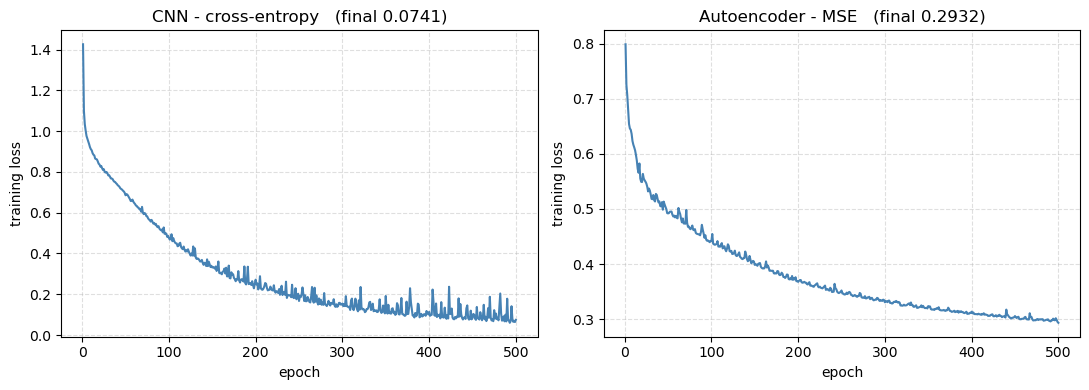
\includegraphics[width=\textwidth]{figures/part2/learning_curve.png}
    \caption{Learning curves of 1D CNN feature extractor (\textbf{Fig. \ref{fig:cnn_extractor}}) and Autoencoder (\textbf{Fig. \ref{fig:autoencoder_flow}}).}
    \label{fig:learning_curves}
\end{figure}